\documentclass[a4paper, 12pt]{article}
\usepackage{graphicx}
\usepackage{listings}
\usepackage{tikz}
\usepackage{amssymb}
\usetikzlibrary{automata, positioning, arrows}


\setlength\parindent{24pt}

\lstset{language=python,breaklines=true, frame=single}
\tikzset{
        ->,  % makes the edges directed
        %>=stealth’, % makes the arrow heads bold
        node distance=7cm, % specifies the minimum distance between two nodes. Change if n
        every state/.style={thick, fill=gray!10}, % sets the properties for each ’state’ n
        initial text=$ $, % sets the text that appears on the start arrow
        }

\begin{document}
\begin{figure}
    \centering
    
\includegraphics[width=1\textwidth]{Logo}
\end{figure}

\title{CPS3233 Assignment Report}
\author{Manwel Bugeja}
\date{\today}
\maketitle
  
\tableofcontents
\newpage

\section{Elevator System Specification}
In this section, the specifications of the elevator system are expressed in several different formal notations. The notations are Finite State Automata (FSAs), Regular Expressions (RE), Timed Automata (TAs) and Duration Calculus (DC). From the ones listed, TAs and DC are the capable of expressing timed events. \\

\subsection{Finite State Automata}
A finite state automata was designed to describe the elevator system. The formal definition of the state machine can be seen in listing \ref{lst:FSA}. The lift can be in one of three states: Idle, Loading or Moving. Idle is when the lift is not moving and has its door closed. Loading when the lift is not moving but has the doors open. Moving is when the lift is moving either up or down. Note that a 'bad' state could be added for when the lift is moving and has the doors open as the lift should never be in this state.
This FSA can be seen visually in \ref{fig:FSA}. \\



\begin{lstlisting}[
caption={FSA definition}
\label{lst:FSA}
]
M = {
{Idle, Loading, Moving},
{openDoor, closeDoor, stop, goUp, goDown},
{
    Idle, openDoor -> Loading,
    Idle, goUp -> Moving,
    Idle, goDown -> Moving,
    Loading, closeDoor -> Idle,
    Moving, stop -> Idle
},
Idle,
{}
}
\end{lstlisting}





\begin{figure}[h] % ’ht’ tells LaTeX to place the figure ’here’ or at the top of the page
    \centering % centers the figure
    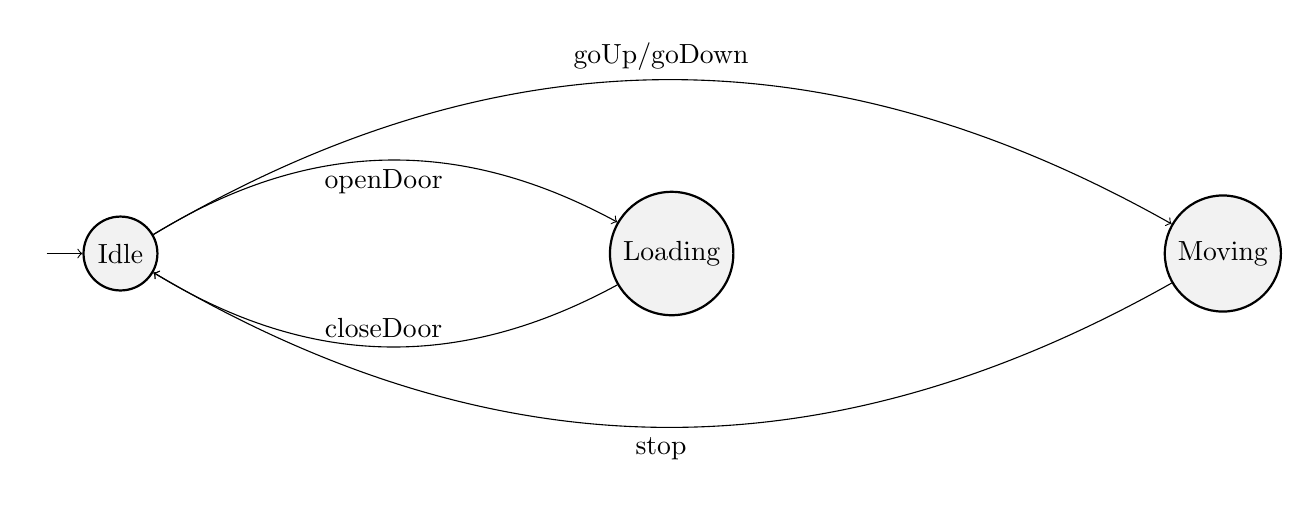
\begin{tikzpicture}
        % tikz code goes here
        \node[state, initial] (Idle) {Idle};
        \node[state, right of=Idle] (Loading) {Loading};
        \node[state, right of=Loading] (Moving) {Moving};
        
        \draw (Idle) edge[bend left, below] node{openDoor} (Loading);
        \draw (Loading) edge[bend left, above] node{closeDoor} (Idle);
       	\draw (Idle) edge[bend left, above] node{goUp/goDown} (Moving);
	\draw (Moving) edge[bend left, below] node{stop} (Idle);
        
    \end{tikzpicture}
    \caption{FSA figure}
    \label{fig:FSA}
\end{figure}


\subsection{Regular Expressions}
The lift system was also expressed via regular expressions. This RE can be seen in listing \ref{lst:RE}. The RE starts of with a series of \textit{openDoor} and \textit{closeDoor} actions which must occur consecutively. This is done so that when the lift moves to the next stage in the RE, the door is always closed, since the lift cannot move with its door open. \\

Next, the RE verifiers that the lift goes an arbitrary number of steps up or down (depending on what the user decided) followed by a stop. The \textit{stop} is there to make sure the lift is not moving when the progress move back to the open/close door part of the expression. \\

An example run of the elevator is:
\texttt{openDoor > closeDoor > goUp > goUp > stop > openDoor > closeDoor > openDoor > closeDoor > goDown > stop}.
This run through is correct according to the RE provided. 

\begin{lstlisting}[
caption={RE definition}
\label{lst:RE}
]
((openDoor.closeDoor)* (goUp* + goDown*).stop )*

\end{lstlisting}


\subsection{Timed Automata}
For the timed automata, the same state machine above was used with some clocks added to verify time-constrained events. In the formal definition if the automaton, the transition functions where modified to accommodate such changes. The formal specification can be seen in listing \ref{lst:TA}. The transition functions follow the format \texttt{[from, to, letter, clocks reseted, condition]}. \\

Important to note in the automaton is that the alphabet is composed of signals the lift can detect, not buttons a user may push. For example the user may interact with the lift by pushing a floor button. This is not detected by the automaton but the lift then proceeds to close the door (provided that it was open). It is the door closing that the automaton uses to verify the scenario. \\

The first time property that is handled states that "upon a request, after the door closes, the elevator starts moving in less than 3 seconds". When adapted to the provided automaton, this translates to "when the lift is \textit{Idle} (because a floor button was pressed so the door closed), it goes either up or down in less than 3 seconds". This is verified by clock x.

The second time property states that "after the door has been open for 3 seconds, it closes automatically". This implies that when the lift has its doors opened i.e. its in the \textit{Loading} state, it must go to the \textit{Idle} in less than 3 seconds. This is because if a user presses the button in less than 3 seconds, the door will close and if he does not press any button, the door closes automatically. This is verified by clock y. 

\begin{lstlisting}[
caption={TA definition}
\label{lst:TA}
]
M = {
{openDoor, closeDoor, stop, goUp, goDown},
{Idle, Loading, Moving},
{idle},
{x, y},
{
    [ Idle, Loading, openDoor, {}, true ]
    
    [ Idle, Moving, goUp, {}, x<3 ]
    
    [ Idle, Moving, goDown, {y:=0}, x<3 ]
    
    [ Loading, Loading, true]
    
    [ Loading, Idle, closeDoor, {x:=0}, y<3 ]
    
    [ Moving, Idle, stop, {x:=0}, true ]
}
}
\end{lstlisting}

\begin{figure}[h] % ’ht’ tells LaTeX to place the figure ’here’ or at the top of the page
    \centering % centers the figure
    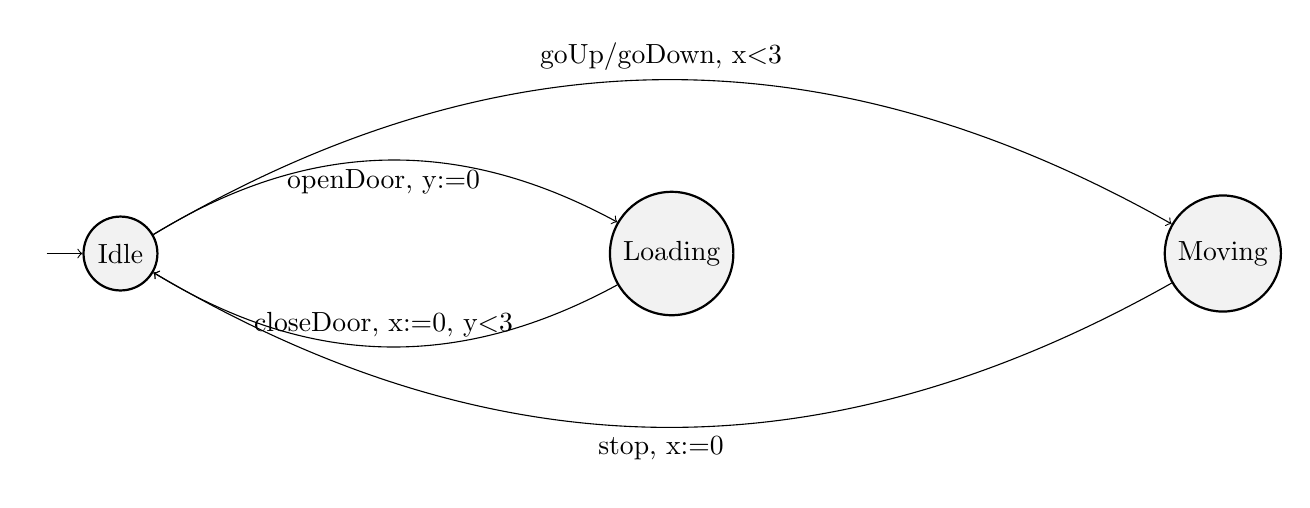
\begin{tikzpicture}
        % tikz code goes here
        \node[state, initial] (Idle) {Idle};
        \node[state, right of=Idle] (Loading) {Loading};
        \node[state, right of=Loading] (Moving) {Moving};
        
        \draw (Idle) edge[bend left, below] node{openDoor, y:=0} (Loading);
        \draw (Loading) edge[bend left, above] node{closeDoor, x:=0, y$<$3} (Idle);
       	\draw (Idle) edge[bend left, above] node{goUp/goDown, x$<$3} (Moving);
	\draw (Moving) edge[bend left, below] node{stop, x:=0} (Idle);
        
    \end{tikzpicture}
    \caption{FSA figure}
    \label{fig:FSA}
\end{figure}

\subsection{Duration Calculus}
For the DC specifications, two formulas where defined, one for each time constrain. The first time constrain states that: "upon a request, after the door closes, the elevator starts moving in less than 3 seconds". This is expressed by the formula:

$$\square [Idle] ; [Loading] ;  [Moving]  \wedge [idle] ; [Loading] ; [Idle] \Rightarrow \int loading < 3$$

The square means that it is checking for all subintervals. Then the pattern the formula is looking for is \textit{Idle}, followed my \textit{Loading}, followed by \textit{Moving}. Then, the expression verifies that the time of loading is less than 3.

The second time constrain says that: after the door has been open for 3 seconds, it closes automatically". The formula describing this is as follows:

$$\square [doorOpen] ; [\neg doorOpen] \Rightarrow \int doorOpen < 3$$

The formula looks for the pattern of an open door followed by a closed door and then verifies that the door was open for less than 3 seconds. 

\section{Runtime Verification}

\section{Model-Based Testing}

\section{Runtime Verification and Testing}

\bibliographystyle{abbrv}
 \bibliography{references}

\end{document}
